%-- einleitung

\section{Experimente}
In diesem Abschnitt wird die entwickelte Bibliothek für Genetische Algorithmen mit dem TSP getestet. Dabei wurden die Resultate mit der Matplotlib-Bibliothek pythonseitig visualisiert.
Diese Verwendung demonstriert die hohe Wiederverwendbarkeit der Projektarbeit.\\
Als Testdatensatz wurde eine Liste an 48 Hauptstädten der USA verwendet \cite{daten}. Diese Daten überzeugten vor allem damit, dass sie einen optimalen Pfad mit Pfaddistanz bereitstellen. Dadurch kann die Qualität der Ergebnisse beurteilt werden.
In den folgenden Experimenten werden die Crossover-Verfahren verglichen, die Populationsgröße und die Mutationswahrscheinlichkeit variiert. Da die Genetischen Algorithmen schwankende Ergebnisse generieren, wurden die Versuche 10 Mal durchgeführt und anschließend ein Mittelwert der fittesten Individuen je Generation gebildet. \\
Zu beachten ist, dass die Distanzen in dem Testdatensatz in Meilen angegeben sind. Weil die Einheit der Distanzen für das TSP irrelevant ist wurde dies nicht korrigiert und im Folgenden vernachlässigt.

\subsection{Experiment 1}
In diesem Experiment wurden die verschiedenen Crossover-Verfahren verglichen. Dabei wurden die Parameter aus Tabelle \ref{tab:e1} verwendet. Die Ergebnisse sind in dem Diagramm \ref{fig:experiment1} zu sehen. 
Die beste Distanz konnte das Order-Crossover-Verfahren erzielen. Allerdings ist auch dessen Distanz mit 55980 Meilen 67\% schlechter als das Optimum von 33351 Meilen. Da durch das automatisierte Testsystem alle Algorithmen auf Korrektheit überprüft wurden, war ein Programmierfehler unwahrscheinlich und ein unbekannter Effekt musste für diese schlechten Ergebnisse verantwortlich sein. Bei der Auswertung der entstehenden Populationen wurde erkannt, dass diese ihre Einzigartigkeit nach wenigen Generationsschritten verlieren. Das bedeutet, dass alle Individuen dasselbe Chromosom in sich tragen und somit die evolutionäre Optimierung scheitert.
Die Ursache für diese Beobachtung ist, dass die eingesetztem Verfahren es ermöglichen, dass sich Chromosome innerhalb von Populationen wiederholen. Tritt dieser Fall auf, so verstärkt sich der Effekt sehr schnell. Aus diesem Grund wurden die Verfahren minimal abgeändert. Das Marriage-Verfahren wählt nun nur noch Eltern aus, die unterschiedlich sind und das Selektions-Verfahren erzeugt ausschließlich distinkte Populationen. Die Ergebnisse dieser Anpassung sind im Experiment 2 zu sehen.

\begin{figure}[H]
\centering
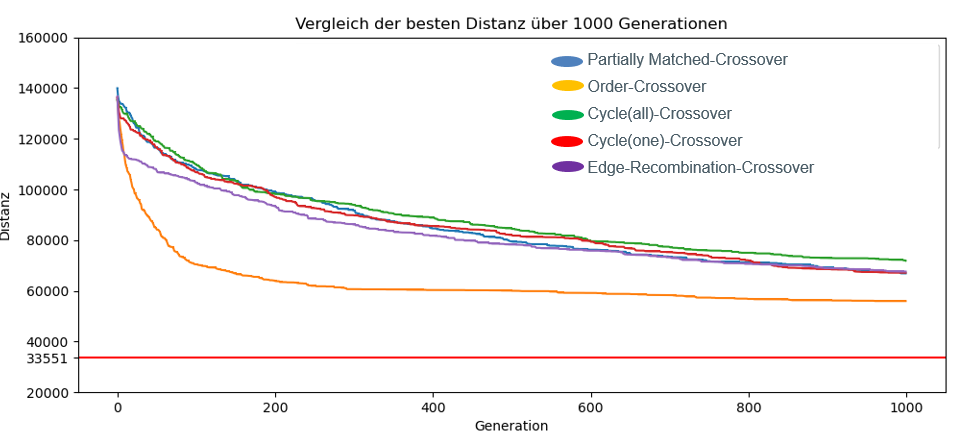
\includegraphics[width=1\textwidth]{img/Vortrag/experiment1.png}
\caption{Ergebnisse des Experiments 1}
\label{fig:experiment1}
\end{figure}

\begin{table}[H]
\centering
\caption{Parameter des Experiments 1}
\begin{tabular}{ll}
Stellschraube & Verfahren \\
\hline
Generationen & 1000 \\
Populationsgröße & 10 \\
Mutations-Verfahren & Delete-And-Shift 5\% \\
Marriage-Verfahren & Roulette \\
Selektions-Verfahren & Survival of the Fittest \\
Crossover & variiert
\end{tabular}
\label{tab:e1}
\end{table}

\subsection{Experiment 2}
In diesem Experiment werden die Resultate aus dem Experiment 1 getestet. Es werden nun die Parameter aus Tabelle \ref{tab:e2} verwendet. Die Ergebnisse sind im Diagramm \ref{fig:experiment2} zu sehen.
Die erreichten Distanzen sind im Allgemeinen deutlich besser geworden, was darauf schließen lässt, dass der Übergang zu distinkten Verfahren korrekt war. Das Order-Crossover-Verfahren erreicht noch immer die beste Distanz mit 48008 Meilen. Dieser Wert ist 43\% schlechter als das Optimum.

\begin{figure}[H]
\centering
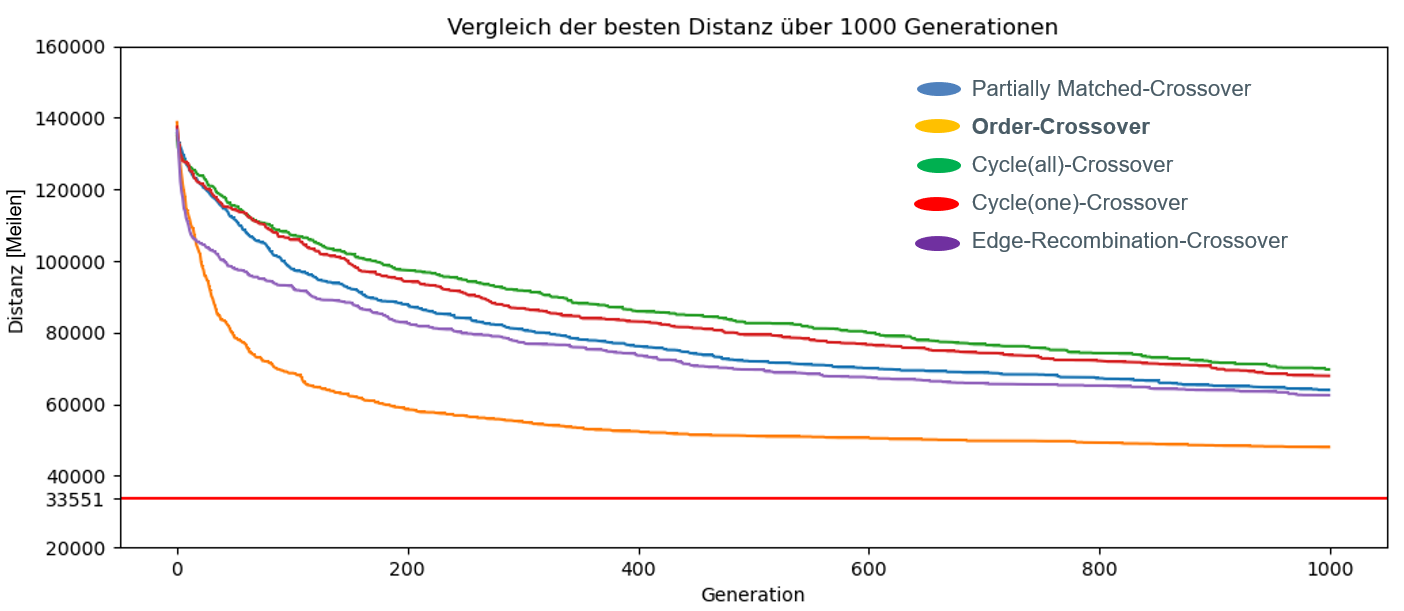
\includegraphics[width=1\textwidth]{img/Vortrag/experiment2.png}
\caption{Ergebnisse des Experiments 2}
\label{fig:experiment2}
\end{figure}

\begin{table}[H]
\centering
\caption{Parameter des Experiments 2}
\begin{tabular}{ll}
Stellschraube & Verfahren \\
\hline
Generationen & 1000 \\
Populationsgröße & 10 \\
Mutations-Verfahren & Delete-And-Shift 5\% \\
Marriage-Verfahren & Roulette Distinkt \\
Selektions-Verfahren & Survival of the Fittest Distinkt \\
Crossover & variiert
\end{tabular}
\label{tab:e2}
\end{table}

\subsection{Experiment 3}
In diesem Experiment wird die Populationsgröße angepasst. Als Crossover-Verfahren wird nun das Order-Crossover-Verfahren eingesetzt. Dieses konnte in Experiment 2 am meisten überzeugen.
Die Parameter sind in Tabelle \ref{tab:e3} zu sehen und die Ergebnisse in Diagramm \ref{fig:experiment3}. Erstaunlich ist, dass eine Populationsgröße von unter 150 zu sehr schlechten Ergebnissen führt. Die Wahl einer Population mit einer Größe von 300 Individuen führt mit einer Distanz von 36520 Meilen zu dem besten Ergebnis und ist nur 8,8\% schlechter als das Optimum. Die Erkenntnis, die daraus gewonnen werden kann ist, dass die bis zu diesem Experiment gewählten Populationsgrößen viel zu gering waren und der Vergleich der Crossover-Verfahren mit einer höheren Populationsgröße wiederholt werden muss.

\begin{figure}[H]
\centering
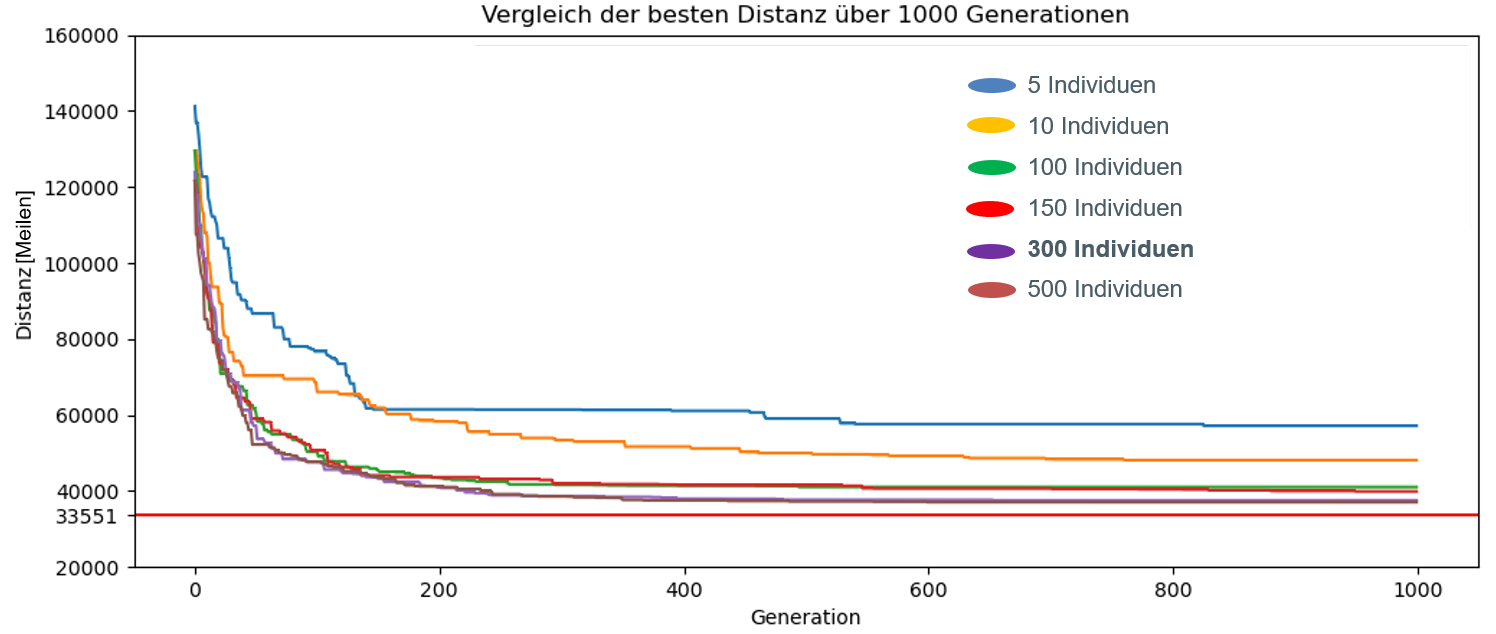
\includegraphics[width=1\textwidth]{img/Vortrag/experiment3.png}
\caption{Ergebnisse des Experiments 3}
\label{fig:experiment3}
\end{figure}

\begin{table}[H]
\centering
\caption{Parameter des Experiments 3}
\begin{tabular}{ll}
Stellschraube & Verfahren \\
\hline
Generationen & 1000 \\
Populationsgröße & variiert \\
Mutations-Verfahren & Delete-And-Shift 5\% \\
Marriage-Verfahren & Roulette Distinkt \\
Selektions-Verfahren & Survival of the Fittest Distinkt \\
Crossover & Order
\end{tabular}
\label{tab:e3}
\end{table}

\subsection{Experiment 4}
In diesem Experiment werden wiederum die Crossover-Verfahren verglichen. Jedoch werden die Erfahrungen der letzten Experimente beachtet und eine Populationsgröße von 300 gewählt sowie distinkte Verfahren eingesetzt.
Die Parametereinstellungen sind in Tabelle \ref{tab:e4} zusammengefasst und führen zu den Resultaten im Diagramm \ref{fig:experiment4}. Nun ist das Edge-Recombination-Verfahren das beste Crossover-Verfahren. Es wird eine Distanz von 34669 Meilen erreicht, was nur 3,3\% schlechter ist als das Optimum von 33551 Meilen. Dieses Resultat überrascht wenig, weil es sich bei dem Edge-Recombination-Verfahren um ein kantenbasiertes Verfahren handelt und im TSP die Kanten die Distanz ergeben.

\begin{figure}[H]
\centering
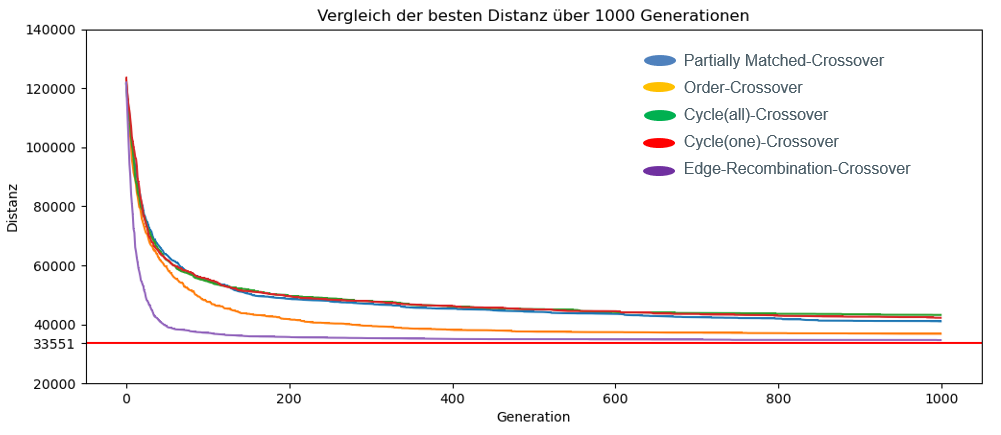
\includegraphics[width=1\textwidth]{img/Vortrag/experiment4.png}
\caption{Ergebnisse des Experiments 4}
\label{fig:experiment4}
\end{figure}

\begin{table}[H]
\centering
\caption{Parameter des Experiments 4}
\begin{tabular}{ll}
Stellschraube & Verfahren \\
\hline
Generationen & 1000 \\
Populationsgröße & 300 \\
Mutations-Verfahren & Delete-And-Shift 5\% \\
Marriage-Verfahren & Roulette Distinkt \\
Selektions-Verfahren & Survival of the Fittest Distinkt \\
Crossover & variiert
\end{tabular}
\label{tab:e4}
\end{table}

\subsection{Experiment 5}
In diesem Experiment wird die Mutationsrate variiert. Die gewählten Parameter sind in Tabelle \ref{tab:e5} zu sehen und die Ergebnisse im Diagramm \ref{fig:experiment5}. Zu sehen ist, dass die Mutationsrate nur einen geringen Effekt auf die Resultate hat. 
Eine Mutationsrate von 10\% führt zu dem besten Ergebnis von 34663 Meilen und stellt somit kaum eine Veränderung zu der bisher gewählten Mutationsrate von 5\% dar. Dies liegt daran, dass das gewählte Mutations-Verfahren nur eine schwache Mutation durchführt. Durch eine stärkere Mutation könnte der Effekt dieses Verfahrensabschnitts womöglich verstärkt werden. Allerdings sind die erzielten Distanzen auch mit diesem Mutations-Verfahren auf einem sehr hohen Niveau. Aus diesem Grund wurden keine weiteren Mutations-Verfahren getestet.

\begin{figure}[H]
\centering
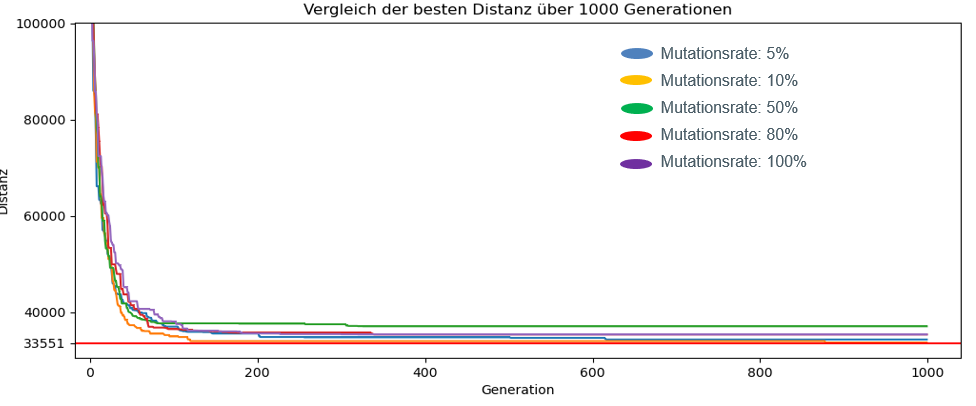
\includegraphics[width=1\textwidth]{img/Vortrag/experiment5.png}
\caption{Ergebnisse des Experiments 5}
\label{fig:experiment5}
\end{figure}

\begin{table}[H]
\centering
\caption{Parameter des Experiments 5}
\begin{tabular}{ll}
Stellschraube & Verfahren \\
\hline
Generationen & 1000 \\
Populationsgröße & 300 \\
Mutations-Verfahren & Delete-And-Shift variiert\% \\
Marriage-Verfahren & Roulette Distinkt \\
Selektions-Verfahren & Survival of the Fittest Distinkt \\
Crossover & Edge-Recombination
\end{tabular}
\label{tab:e5}
\end{table}

\subsection{Experiment 6}
Dieses Experiment fasst die Resultate der bisher durchgeführten Experimente zusammen und vergleicht die Crossover-Verfahren mit den gefundenen optimalen Parametereinstellungen aus Tabelle \ref{tab:e6}.
Das Edge-Recombination-Verfahren überzeugt mit einer Distanz von 34372 Meilen. Dieses Ergebnis ist lediglich 2,4\% schlechter als das optimale Ergebnis von 33551 Meilen. 
\begin{figure}[H]
\centering
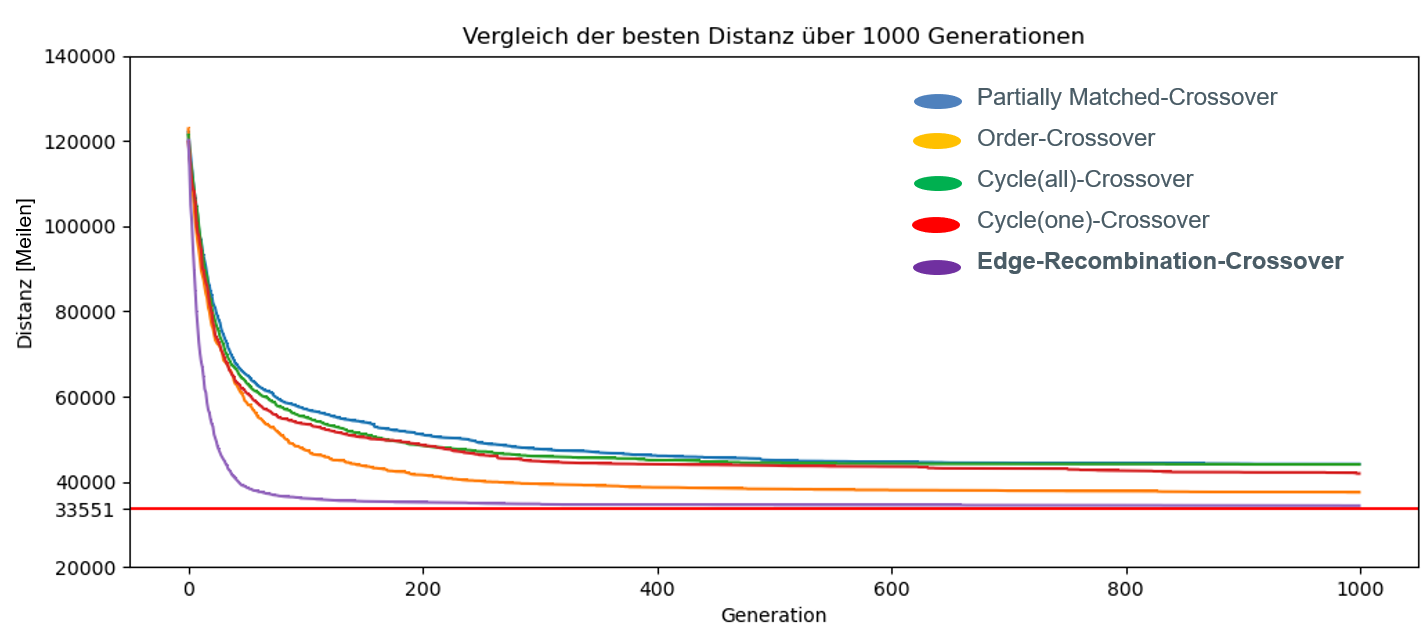
\includegraphics[width=1\textwidth]{img/Vortrag/experiment6.png}
\caption{Ergebnisse des Experiments 6}
\label{fig:experiment6}
\end{figure}

\begin{table}[H]
\centering
\caption{Parameter des Experiments 6}
\begin{tabular}{ll}
Stellschraube & Verfahren \\
\hline
Generationen & 1000 \\
Populationsgröße & 300 \\
Mutations-Verfahren & Delete-And-Shift 10\% \\
Marriage-Verfahren & Roulette Distinkt \\
Selektions-Verfahren & Survival of the Fittest Distinkt \\
Crossover & variiert
\end{tabular}
\label{tab:e6}
\end{table}

\subsection{Experiment 7}
In diesem Experiment wird der erzeugte Rundlauf mit dem optimalen Rundlauf verglichen. Dazu ist in Grafik \ref{fig:experiment71} der gegebene optimale Rundlauf und im Gegensatz dazu ein generierter Rundlauf in Grafik \ref{fig:experiment72} zu sehen. Für diese Simulation wurden die Parameter aus Tabelle \ref{tab:e7} gewählt. Diese Darstellung liefert allerdings nur wenige neue Erkenntnisse. Das generierte Ergebnis ist ein lokales Minima und weist viele Ähnlichkeiten zu dem optimalen Rundlauf auf, jedoch auch viele Unterschiede. Es ist dennoch interessant das Ergebnis der Arbeit betrachten zu können.

\begin{figure}
	\centering
	\begin{subfigure}[Optimum]{0.49\textwidth}
		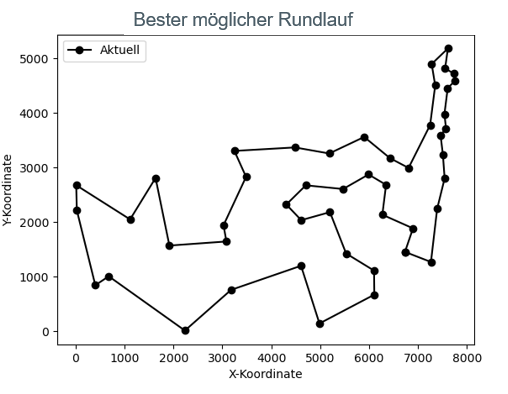
\includegraphics[width=\textwidth]{img/Vortrag/experiment7_1.png}
		\caption{Optimaler Rundlauf}
		\label{fig:experiment71}
	\end{subfigure}
	\begin{subfigure}[Simulation]{0.49\textwidth}
		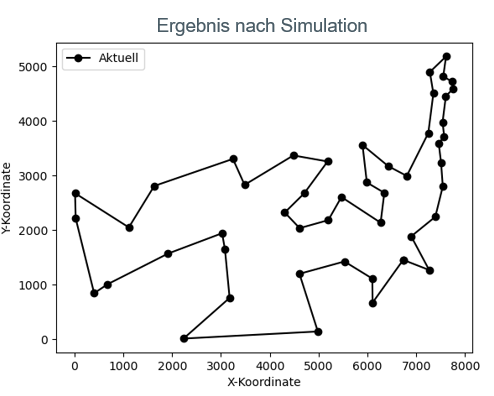
\includegraphics[width=\textwidth]{img/Vortrag/experiment7_2.png}
		\caption{Rundlauf nach Simulation}
		\label{fig:experiment72}
	\end{subfigure}
\caption{Ergebnisse des Experiments 7}
\label{fig:experiment7}
\end{figure}

\begin{table}[H]
\centering
\caption{Parameter des Experiments 7}
\begin{tabular}{ll}
Stellschraube & Verfahren \\
\hline
Generationen & 1000 \\
Populationsgröße & 300 \\
Mutations-Verfahren & Delete-And-Shift 10\% \\
Marriage-Verfahren & Roulette Distinkt \\
Selektions-Verfahren & Survival of the Fittest Distinkt \\
Crossover & Edge-Recombination
\end{tabular}
\label{tab:e7}
\end{table}

%--